\documentclass[letterpaper,12pt]{article}
\usepackage[margin=14mm,top=18mm,bottom=17mm,headheight=14pt]{geometry}
\pdfmapfile{+cm.map}\pdfmapfile{+cmextra.map}
\usepackage{tikz,fancyhdr,amsmath,amssymb}
\usetikzlibrary{arrows.meta,patterns}
\pagestyle{fancy}\fancyhf{}\renewcommand{\headrulewidth}{0pt}
\fancyhead[L]{\small Week 49 / Four-tower differences / Grades 4--5}
\fancyfoot[L]{\small Bellingham Math Circle / Week 49 / F49-45-v2}
\fancyfoot[R]{\small\thepage}
\setlength{\parindent}{0pt}\setlength{\parskip}{0pt}
\begin{document}
\noindent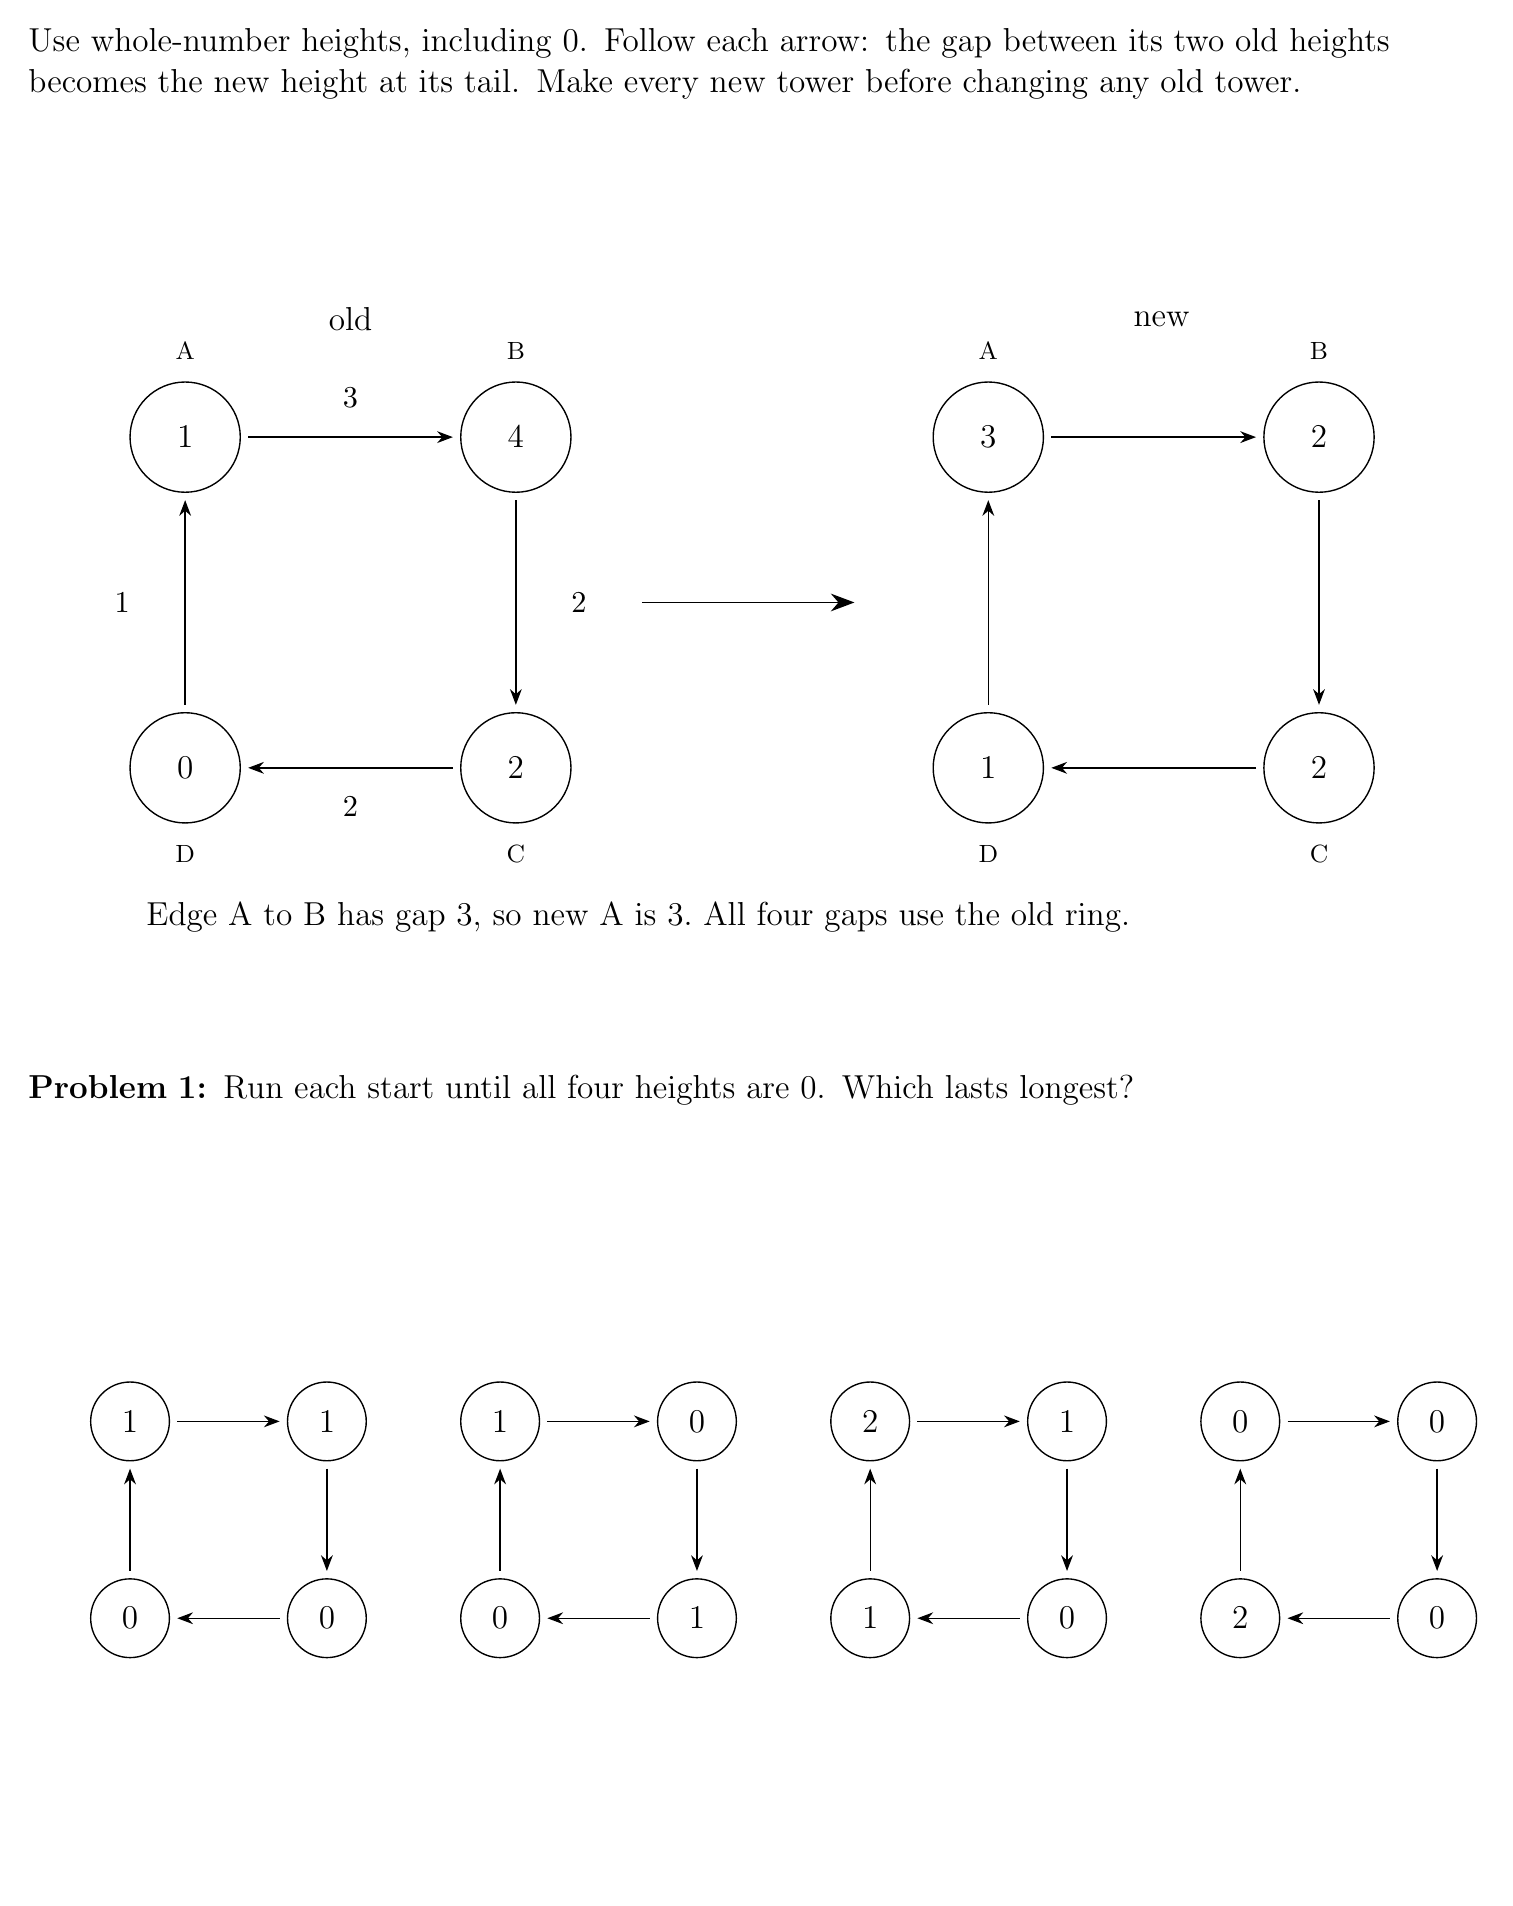
\begin{tikzpicture}[x=1mm,y=-1mm,line width=.5pt]
\path[use as bounding box] (0,0) rectangle (185,235);
\node[anchor=north west,inner sep=0pt,text width=180mm,font=\fontsize{12}{15}\selectfont] at (0,0) {Use whole-number heights, including 0. Follow each arrow: the gap between its two old heights becomes the new height at its tail. Make every new tower before changing any old tower.};
\node[anchor=center,inner sep=1pt,font=\fontsize{12}{14}\selectfont] at (41,37) {old};
\node[anchor=center,inner sep=1pt,font=\fontsize{12}{14}\selectfont] at (144,37) {new};
\draw[-{Stealth[length=2mm]}] (28.0,52.0) -- (54.0,52.0);
\node[anchor=center,inner sep=1pt,font=\fontsize{11}{13}\selectfont] at (41.0,47.0) {3};
\draw[-{Stealth[length=2mm]}] (62.0,60.0) -- (62.0,86.0);
\node[anchor=center,inner sep=1pt,font=\fontsize{11}{13}\selectfont] at (70.0,73.0) {2};
\draw[-{Stealth[length=2mm]}] (54.0,94.0) -- (28.0,94.0);
\node[anchor=center,inner sep=1pt,font=\fontsize{11}{13}\selectfont] at (41.0,99.0) {2};
\draw[-{Stealth[length=2mm]}] (20.0,86.0) -- (20.0,60.0);
\node[anchor=center,inner sep=1pt,font=\fontsize{11}{13}\selectfont] at (12.0,73.0) {1};
\draw[fill=white] (20,52) circle (7);
\node[anchor=center,inner sep=1pt,font=\fontsize{9}{11}\selectfont] at (20,41) {A};
\node[anchor=center,inner sep=1pt,font=\fontsize{13}{15}\selectfont] at (20,52) {1};
\draw[fill=white] (62,52) circle (7);
\node[anchor=center,inner sep=1pt,font=\fontsize{9}{11}\selectfont] at (62,41) {B};
\node[anchor=center,inner sep=1pt,font=\fontsize{13}{15}\selectfont] at (62,52) {4};
\draw[fill=white] (62,94) circle (7);
\node[anchor=center,inner sep=1pt,font=\fontsize{9}{11}\selectfont] at (62,105) {C};
\node[anchor=center,inner sep=1pt,font=\fontsize{13}{15}\selectfont] at (62,94) {2};
\draw[fill=white] (20,94) circle (7);
\node[anchor=center,inner sep=1pt,font=\fontsize{9}{11}\selectfont] at (20,105) {D};
\node[anchor=center,inner sep=1pt,font=\fontsize{13}{15}\selectfont] at (20,94) {0};
\draw[-{Stealth[length=3mm]}] (78,73) -- (105,73);
\draw[-{Stealth[length=2mm]}] (130.0,52.0) -- (156.0,52.0);
\draw[-{Stealth[length=2mm]}] (164.0,60.0) -- (164.0,86.0);
\draw[-{Stealth[length=2mm]}] (156.0,94.0) -- (130.0,94.0);
\draw[-{Stealth[length=2mm]}] (122.0,86.0) -- (122.0,60.0);
\draw[fill=white] (122,52) circle (7);
\node[anchor=center,inner sep=1pt,font=\fontsize{9}{11}\selectfont] at (122,41) {A};
\node[anchor=center,inner sep=1pt,font=\fontsize{13}{15}\selectfont] at (122,52) {3};
\draw[fill=white] (164,52) circle (7);
\node[anchor=center,inner sep=1pt,font=\fontsize{9}{11}\selectfont] at (164,41) {B};
\node[anchor=center,inner sep=1pt,font=\fontsize{13}{15}\selectfont] at (164,52) {2};
\draw[fill=white] (164,94) circle (7);
\node[anchor=center,inner sep=1pt,font=\fontsize{9}{11}\selectfont] at (164,105) {C};
\node[anchor=center,inner sep=1pt,font=\fontsize{13}{15}\selectfont] at (164,94) {2};
\draw[fill=white] (122,94) circle (7);
\node[anchor=center,inner sep=1pt,font=\fontsize{9}{11}\selectfont] at (122,105) {D};
\node[anchor=center,inner sep=1pt,font=\fontsize{13}{15}\selectfont] at (122,94) {1};
\node[anchor=north west,inner sep=0pt,text width=180mm,font=\fontsize{12}{15}\selectfont] at (15,111) {Edge A to B has gap 3, so new A is 3.\ All four gaps use the old ring.};
\node[anchor=north west,inner sep=0pt,text width=180mm,font=\fontsize{13}{16}\selectfont] at (0,133) {\textbf{Problem 1:} Run each start until all four heights are 0. Which lasts longest?};
\draw[-{Stealth[length=2mm]}] (19.0,177.0) -- (32.0,177.0);
\draw[-{Stealth[length=2mm]}] (38.0,183.0) -- (38.0,196.0);
\draw[-{Stealth[length=2mm]}] (32.0,202.0) -- (19.0,202.0);
\draw[-{Stealth[length=2mm]}] (13.0,196.0) -- (13.0,183.0);
\draw[fill=white] (13,177) circle (5);
\node[anchor=center,inner sep=1pt,font=\fontsize{13}{15}\selectfont] at (13,177) {1};
\draw[fill=white] (38,177) circle (5);
\node[anchor=center,inner sep=1pt,font=\fontsize{13}{15}\selectfont] at (38,177) {1};
\draw[fill=white] (38,202) circle (5);
\node[anchor=center,inner sep=1pt,font=\fontsize{13}{15}\selectfont] at (38,202) {0};
\draw[fill=white] (13,202) circle (5);
\node[anchor=center,inner sep=1pt,font=\fontsize{13}{15}\selectfont] at (13,202) {0};
\draw[-{Stealth[length=2mm]}] (66.0,177.0) -- (79.0,177.0);
\draw[-{Stealth[length=2mm]}] (85.0,183.0) -- (85.0,196.0);
\draw[-{Stealth[length=2mm]}] (79.0,202.0) -- (66.0,202.0);
\draw[-{Stealth[length=2mm]}] (60.0,196.0) -- (60.0,183.0);
\draw[fill=white] (60,177) circle (5);
\node[anchor=center,inner sep=1pt,font=\fontsize{13}{15}\selectfont] at (60,177) {1};
\draw[fill=white] (85,177) circle (5);
\node[anchor=center,inner sep=1pt,font=\fontsize{13}{15}\selectfont] at (85,177) {0};
\draw[fill=white] (85,202) circle (5);
\node[anchor=center,inner sep=1pt,font=\fontsize{13}{15}\selectfont] at (85,202) {1};
\draw[fill=white] (60,202) circle (5);
\node[anchor=center,inner sep=1pt,font=\fontsize{13}{15}\selectfont] at (60,202) {0};
\draw[-{Stealth[length=2mm]}] (113.0,177.0) -- (126.0,177.0);
\draw[-{Stealth[length=2mm]}] (132.0,183.0) -- (132.0,196.0);
\draw[-{Stealth[length=2mm]}] (126.0,202.0) -- (113.0,202.0);
\draw[-{Stealth[length=2mm]}] (107.0,196.0) -- (107.0,183.0);
\draw[fill=white] (107,177) circle (5);
\node[anchor=center,inner sep=1pt,font=\fontsize{13}{15}\selectfont] at (107,177) {2};
\draw[fill=white] (132,177) circle (5);
\node[anchor=center,inner sep=1pt,font=\fontsize{13}{15}\selectfont] at (132,177) {1};
\draw[fill=white] (132,202) circle (5);
\node[anchor=center,inner sep=1pt,font=\fontsize{13}{15}\selectfont] at (132,202) {0};
\draw[fill=white] (107,202) circle (5);
\node[anchor=center,inner sep=1pt,font=\fontsize{13}{15}\selectfont] at (107,202) {1};
\draw[-{Stealth[length=2mm]}] (160.0,177.0) -- (173.0,177.0);
\draw[-{Stealth[length=2mm]}] (179.0,183.0) -- (179.0,196.0);
\draw[-{Stealth[length=2mm]}] (173.0,202.0) -- (160.0,202.0);
\draw[-{Stealth[length=2mm]}] (154.0,196.0) -- (154.0,183.0);
\draw[fill=white] (154,177) circle (5);
\node[anchor=center,inner sep=1pt,font=\fontsize{13}{15}\selectfont] at (154,177) {0};
\draw[fill=white] (179,177) circle (5);
\node[anchor=center,inner sep=1pt,font=\fontsize{13}{15}\selectfont] at (179,177) {0};
\draw[fill=white] (179,202) circle (5);
\node[anchor=center,inner sep=1pt,font=\fontsize{13}{15}\selectfont] at (179,202) {0};
\draw[fill=white] (154,202) circle (5);
\node[anchor=center,inner sep=1pt,font=\fontsize{13}{15}\selectfont] at (154,202) {2};
\end{tikzpicture}
\newpage
\noindent\begin{tikzpicture}[x=1mm,y=-1mm,line width=.5pt]
\path[use as bounding box] (0,0) rectangle (185,235);
\node[anchor=north west,inner sep=0pt,text width=180mm,font=\fontsize{13}{16}\selectfont] at (0,0) {\textbf{Problem 2:} Choose starting heights from 0 to 5. Find a ring that lasts as many moves as you can. Count the move that first makes all four heights 0.};
\node[anchor=north west,inner sep=0pt,text width=180mm,font=\fontsize{11}{14}\selectfont] at (0,25) {An all-zero start takes 0 moves. Use these big mats for all four-station starts.};
\node[anchor=center,inner sep=1pt,font=\fontsize{12}{14}\selectfont] at (46,43) {old};
\node[anchor=center,inner sep=1pt,font=\fontsize{12}{14}\selectfont] at (139,43) {new};
\draw[-{Stealth[length=2mm]}] (41.0,71.0) -- (51.0,71.0);
\draw[-{Stealth[length=2mm]}] (72.0,92.0) -- (72.0,102.0);
\draw[-{Stealth[length=2mm]}] (51.0,123.0) -- (41.0,123.0);
\draw[-{Stealth[length=2mm]}] (20.0,102.0) -- (20.0,92.0);
\draw[fill=white,rounded corners=1mm] (0,51) rectangle ++(40,40);
\node[anchor=center,inner sep=1pt,font=\fontsize{9}{11}\selectfont] at (20,47) {A};
\draw[fill=white,rounded corners=1mm] (52,51) rectangle ++(40,40);
\node[anchor=center,inner sep=1pt,font=\fontsize{9}{11}\selectfont] at (72,47) {B};
\draw[fill=white,rounded corners=1mm] (52,103) rectangle ++(40,40);
\node[anchor=center,inner sep=1pt,font=\fontsize{9}{11}\selectfont] at (72,147) {C};
\draw[fill=white,rounded corners=1mm] (0,103) rectangle ++(40,40);
\node[anchor=center,inner sep=1pt,font=\fontsize{9}{11}\selectfont] at (20,147) {D};
\draw[-{Stealth[length=2mm]}] (134.0,71.0) -- (144.0,71.0);
\draw[-{Stealth[length=2mm]}] (165.0,92.0) -- (165.0,102.0);
\draw[-{Stealth[length=2mm]}] (144.0,123.0) -- (134.0,123.0);
\draw[-{Stealth[length=2mm]}] (113.0,102.0) -- (113.0,92.0);
\draw[fill=white,rounded corners=1mm] (93,51) rectangle ++(40,40);
\node[anchor=center,inner sep=1pt,font=\fontsize{9}{11}\selectfont] at (113,47) {A};
\draw[fill=white,rounded corners=1mm] (145,51) rectangle ++(40,40);
\node[anchor=center,inner sep=1pt,font=\fontsize{9}{11}\selectfont] at (165,47) {B};
\draw[fill=white,rounded corners=1mm] (145,103) rectangle ++(40,40);
\node[anchor=center,inner sep=1pt,font=\fontsize{9}{11}\selectfont] at (165,147) {C};
\draw[fill=white,rounded corners=1mm] (93,103) rectangle ++(40,40);
\node[anchor=center,inner sep=1pt,font=\fontsize{9}{11}\selectfont] at (113,147) {D};
\draw[] (20,176) rectangle ++(14,11);
\node[anchor=center,inner sep=1pt,font=\fontsize{12}{14}\selectfont] at (27,181.5) {};
\node[anchor=center,inner sep=1pt,font=\fontsize{9}{11}\selectfont] at (27,172) {A};
\draw[] (34,176) rectangle ++(14,11);
\node[anchor=center,inner sep=1pt,font=\fontsize{12}{14}\selectfont] at (41,181.5) {};
\node[anchor=center,inner sep=1pt,font=\fontsize{9}{11}\selectfont] at (41,172) {B};
\draw[] (48,176) rectangle ++(14,11);
\node[anchor=center,inner sep=1pt,font=\fontsize{12}{14}\selectfont] at (55,181.5) {};
\node[anchor=center,inner sep=1pt,font=\fontsize{9}{11}\selectfont] at (55,172) {C};
\draw[] (62,176) rectangle ++(14,11);
\node[anchor=center,inner sep=1pt,font=\fontsize{12}{14}\selectfont] at (69,181.5) {};
\node[anchor=center,inner sep=1pt,font=\fontsize{9}{11}\selectfont] at (69,172) {D};
\node[anchor=north west,inner sep=0pt,text width=85mm,font=\fontsize{12}{15}\selectfont] at (97,176) {Moves to zero: \rule{17mm}{.3pt}};
\draw[] (20,213) rectangle ++(14,11);
\node[anchor=center,inner sep=1pt,font=\fontsize{12}{14}\selectfont] at (27,218.5) {};
\node[anchor=center,inner sep=1pt,font=\fontsize{9}{11}\selectfont] at (27,209) {A};
\draw[] (34,213) rectangle ++(14,11);
\node[anchor=center,inner sep=1pt,font=\fontsize{12}{14}\selectfont] at (41,218.5) {};
\node[anchor=center,inner sep=1pt,font=\fontsize{9}{11}\selectfont] at (41,209) {B};
\draw[] (48,213) rectangle ++(14,11);
\node[anchor=center,inner sep=1pt,font=\fontsize{12}{14}\selectfont] at (55,218.5) {};
\node[anchor=center,inner sep=1pt,font=\fontsize{9}{11}\selectfont] at (55,209) {C};
\draw[] (62,213) rectangle ++(14,11);
\node[anchor=center,inner sep=1pt,font=\fontsize{12}{14}\selectfont] at (69,218.5) {};
\node[anchor=center,inner sep=1pt,font=\fontsize{9}{11}\selectfont] at (69,209) {D};
\node[anchor=north west,inner sep=0pt,text width=85mm,font=\fontsize{12}{15}\selectfont] at (97,213) {Moves to zero: \rule{17mm}{.3pt}};
\end{tikzpicture}
\newpage
\noindent\begin{tikzpicture}[x=1mm,y=-1mm,line width=.5pt]
\path[use as bounding box] (0,0) rectangle (185,235);
\node[anchor=north west,inner sep=0pt,text width=180mm,font=\fontsize{13}{16}\selectfont] at (0,0) {\textbf{Problem 3:} Could each ring be the result of one move? Find an old ring that makes it, or explain why no old ring can work.};
\draw[-{Stealth[length=2mm]}] (37.0,53.0) -- (59.0,53.0);
\draw[-{Stealth[length=2mm]}] (68.0,62.0) -- (68.0,84.0);
\draw[-{Stealth[length=2mm]}] (59.0,93.0) -- (37.0,93.0);
\draw[-{Stealth[length=2mm]}] (28.0,84.0) -- (28.0,62.0);
\draw[fill=white] (28,53) circle (8);
\node[anchor=center,inner sep=1pt,font=\fontsize{9}{11}\selectfont] at (28,41) {A};
\node[anchor=center,inner sep=1pt,font=\fontsize{13}{15}\selectfont] at (28,53) {2};
\draw[fill=white] (68,53) circle (8);
\node[anchor=center,inner sep=1pt,font=\fontsize{9}{11}\selectfont] at (68,41) {B};
\node[anchor=center,inner sep=1pt,font=\fontsize{13}{15}\selectfont] at (68,53) {0};
\draw[fill=white] (68,93) circle (8);
\node[anchor=center,inner sep=1pt,font=\fontsize{9}{11}\selectfont] at (68,105) {C};
\node[anchor=center,inner sep=1pt,font=\fontsize{13}{15}\selectfont] at (68,93) {2};
\draw[fill=white] (28,93) circle (8);
\node[anchor=center,inner sep=1pt,font=\fontsize{9}{11}\selectfont] at (28,105) {D};
\node[anchor=center,inner sep=1pt,font=\fontsize{13}{15}\selectfont] at (28,93) {0};
\draw[-{Stealth[length=2mm]}] (129.0,53.0) -- (151.0,53.0);
\draw[-{Stealth[length=2mm]}] (160.0,62.0) -- (160.0,84.0);
\draw[-{Stealth[length=2mm]}] (151.0,93.0) -- (129.0,93.0);
\draw[-{Stealth[length=2mm]}] (120.0,84.0) -- (120.0,62.0);
\draw[fill=white] (120,53) circle (8);
\node[anchor=center,inner sep=1pt,font=\fontsize{9}{11}\selectfont] at (120,41) {A};
\node[anchor=center,inner sep=1pt,font=\fontsize{13}{15}\selectfont] at (120,53) {1};
\draw[fill=white] (160,53) circle (8);
\node[anchor=center,inner sep=1pt,font=\fontsize{9}{11}\selectfont] at (160,41) {B};
\node[anchor=center,inner sep=1pt,font=\fontsize{13}{15}\selectfont] at (160,53) {1};
\draw[fill=white] (160,93) circle (8);
\node[anchor=center,inner sep=1pt,font=\fontsize{9}{11}\selectfont] at (160,105) {C};
\node[anchor=center,inner sep=1pt,font=\fontsize{13}{15}\selectfont] at (160,93) {1};
\draw[fill=white] (120,93) circle (8);
\node[anchor=center,inner sep=1pt,font=\fontsize{9}{11}\selectfont] at (120,105) {D};
\node[anchor=center,inner sep=1pt,font=\fontsize{13}{15}\selectfont] at (120,93) {0};
\draw[-{Stealth[length=2mm]}] (37.0,147.0) -- (59.0,147.0);
\draw[-{Stealth[length=2mm]}] (68.0,156.0) -- (68.0,178.0);
\draw[-{Stealth[length=2mm]}] (59.0,187.0) -- (37.0,187.0);
\draw[-{Stealth[length=2mm]}] (28.0,178.0) -- (28.0,156.0);
\draw[fill=white] (28,147) circle (8);
\node[anchor=center,inner sep=1pt,font=\fontsize{9}{11}\selectfont] at (28,135) {A};
\node[anchor=center,inner sep=1pt,font=\fontsize{13}{15}\selectfont] at (28,147) {1};
\draw[fill=white] (68,147) circle (8);
\node[anchor=center,inner sep=1pt,font=\fontsize{9}{11}\selectfont] at (68,135) {B};
\node[anchor=center,inner sep=1pt,font=\fontsize{13}{15}\selectfont] at (68,147) {1};
\draw[fill=white] (68,187) circle (8);
\node[anchor=center,inner sep=1pt,font=\fontsize{9}{11}\selectfont] at (68,199) {C};
\node[anchor=center,inner sep=1pt,font=\fontsize{13}{15}\selectfont] at (68,187) {1};
\draw[fill=white] (28,187) circle (8);
\node[anchor=center,inner sep=1pt,font=\fontsize{9}{11}\selectfont] at (28,199) {D};
\node[anchor=center,inner sep=1pt,font=\fontsize{13}{15}\selectfont] at (28,187) {1};
\draw[-{Stealth[length=2mm]}] (129.0,147.0) -- (151.0,147.0);
\draw[-{Stealth[length=2mm]}] (160.0,156.0) -- (160.0,178.0);
\draw[-{Stealth[length=2mm]}] (151.0,187.0) -- (129.0,187.0);
\draw[-{Stealth[length=2mm]}] (120.0,178.0) -- (120.0,156.0);
\draw[fill=white] (120,147) circle (8);
\node[anchor=center,inner sep=1pt,font=\fontsize{9}{11}\selectfont] at (120,135) {A};
\node[anchor=center,inner sep=1pt,font=\fontsize{13}{15}\selectfont] at (120,147) {0};
\draw[fill=white] (160,147) circle (8);
\node[anchor=center,inner sep=1pt,font=\fontsize{9}{11}\selectfont] at (160,135) {B};
\node[anchor=center,inner sep=1pt,font=\fontsize{13}{15}\selectfont] at (160,147) {0};
\draw[fill=white] (160,187) circle (8);
\node[anchor=center,inner sep=1pt,font=\fontsize{9}{11}\selectfont] at (160,199) {C};
\node[anchor=center,inner sep=1pt,font=\fontsize{13}{15}\selectfont] at (160,187) {0};
\draw[fill=white] (120,187) circle (8);
\node[anchor=center,inner sep=1pt,font=\fontsize{9}{11}\selectfont] at (120,199) {D};
\node[anchor=center,inner sep=1pt,font=\fontsize{13}{15}\selectfont] at (120,187) {2};
\end{tikzpicture}
\newpage
\noindent\begin{tikzpicture}[x=1mm,y=-1mm,line width=.5pt]
\path[use as bounding box] (0,0) rectangle (185,235);
\node[anchor=north west,inner sep=0pt,text width=180mm,font=\fontsize{13}{16}\selectfont] at (0,0) {\textbf{Problem 4:} Use the gap rule on both rings. Keep going until the whole ring repeats or becomes all zeros. Does the number of stations change what can happen?};
\draw[-{Stealth[length=2mm]}] (37.0,45.0) -- (51.0,45.0);
\draw[-{Stealth[length=2mm]}] (58.0,52.0) -- (58.0,66.0);
\draw[-{Stealth[length=2mm]}] (51.0,73.0) -- (37.0,73.0);
\draw[-{Stealth[length=2mm]}] (30.0,66.0) -- (30.0,52.0);
\draw[fill=white] (30,45) circle (6);
\node[anchor=center,inner sep=1pt,font=\fontsize{9}{11}\selectfont] at (30,35) {A};
\node[anchor=center,inner sep=1pt,font=\fontsize{13}{15}\selectfont] at (30,45) {1};
\draw[fill=white] (58,45) circle (6);
\node[anchor=center,inner sep=1pt,font=\fontsize{9}{11}\selectfont] at (58,35) {B};
\node[anchor=center,inner sep=1pt,font=\fontsize{13}{15}\selectfont] at (58,45) {0};
\draw[fill=white] (58,73) circle (6);
\node[anchor=center,inner sep=1pt,font=\fontsize{9}{11}\selectfont] at (58,83) {C};
\node[anchor=center,inner sep=1pt,font=\fontsize{13}{15}\selectfont] at (58,73) {0};
\draw[fill=white] (30,73) circle (6);
\node[anchor=center,inner sep=1pt,font=\fontsize{9}{11}\selectfont] at (30,83) {D};
\node[anchor=center,inner sep=1pt,font=\fontsize{13}{15}\selectfont] at (30,73) {0};
\draw[-{Stealth[length=2mm]}] (144.1304951684997,51.26099033699941) -- (151.8695048315003,66.73900966300059);
\draw[-{Stealth[length=2mm]}] (148.0,73.0) -- (134.0,73.0);
\draw[-{Stealth[length=2mm]}] (130.1304951684997,66.73900966300059) -- (137.8695048315003,51.26099033699941);
\draw[fill=white] (141.0,45) circle (6);
\node[anchor=center,inner sep=1pt,font=\fontsize{9}{11}\selectfont] at (141.0,35) {A};
\node[anchor=center,inner sep=1pt,font=\fontsize{13}{15}\selectfont] at (141.0,45) {1};
\draw[fill=white] (155,73) circle (6);
\node[anchor=center,inner sep=1pt,font=\fontsize{9}{11}\selectfont] at (155,83) {B};
\node[anchor=center,inner sep=1pt,font=\fontsize{13}{15}\selectfont] at (155,73) {0};
\draw[fill=white] (127,73) circle (6);
\node[anchor=center,inner sep=1pt,font=\fontsize{9}{11}\selectfont] at (127,83) {C};
\node[anchor=center,inner sep=1pt,font=\fontsize{13}{15}\selectfont] at (127,73) {0};
\node[anchor=center,inner sep=1pt,font=\fontsize{12}{14}\selectfont] at (46,91) {old};
\node[anchor=center,inner sep=1pt,font=\fontsize{12}{14}\selectfont] at (139,91) {new};
\draw[-{Stealth[length=2mm]}] (56.44721359549996,139.89442719099992) -- (61.55278640450004,150.10557280900008);
\draw[-{Stealth[length=2mm]}] (51.0,171.0) -- (41.0,171.0);
\draw[-{Stealth[length=2mm]}] (30.44721359549996,150.10557280900008) -- (35.55278640450004,139.89442719099992);
\draw[fill=white,rounded corners=1mm] (26.0,99) rectangle ++(40,40);
\node[anchor=center,inner sep=1pt,font=\fontsize{9}{11}\selectfont] at (46.0,95) {A};
\draw[fill=white,rounded corners=1mm] (52,151) rectangle ++(40,40);
\node[anchor=center,inner sep=1pt,font=\fontsize{9}{11}\selectfont] at (72,195) {B};
\draw[fill=white,rounded corners=1mm] (0,151) rectangle ++(40,40);
\node[anchor=center,inner sep=1pt,font=\fontsize{9}{11}\selectfont] at (20,195) {C};
\draw[-{Stealth[length=2mm]}] (149.44721359549996,139.89442719099992) -- (154.55278640450004,150.10557280900008);
\draw[-{Stealth[length=2mm]}] (144.0,171.0) -- (134.0,171.0);
\draw[-{Stealth[length=2mm]}] (123.44721359549996,150.10557280900008) -- (128.55278640450004,139.89442719099992);
\draw[fill=white,rounded corners=1mm] (119.0,99) rectangle ++(40,40);
\node[anchor=center,inner sep=1pt,font=\fontsize{9}{11}\selectfont] at (139.0,95) {A};
\draw[fill=white,rounded corners=1mm] (145,151) rectangle ++(40,40);
\node[anchor=center,inner sep=1pt,font=\fontsize{9}{11}\selectfont] at (165,195) {B};
\draw[fill=white,rounded corners=1mm] (93,151) rectangle ++(40,40);
\node[anchor=center,inner sep=1pt,font=\fontsize{9}{11}\selectfont] at (113,195) {C};
\end{tikzpicture}
\newpage
\noindent\begin{tikzpicture}[x=1mm,y=-1mm,line width=.5pt]
\path[use as bounding box] (0,0) rectangle (185,235);
\node[anchor=north west,inner sep=0pt,text width=180mm,font=\fontsize{13}{16}\selectfont] at (0,0) {\textbf{Problem 5:} Replace even heights by E and odd heights by O. Use this two-letter gap rule. Which letter rings are possible after four moves? Explain why you have checked every kind of start.};
\node[anchor=north west,inner sep=0pt,text width=180mm,font=\fontsize{12}{15}\selectfont] at (5,34) {E and E give E.     O and O give E.};
\node[anchor=north west,inner sep=0pt,text width=180mm,font=\fontsize{12}{15}\selectfont] at (5,44) {E and O give O.     O and E give O.};
\draw[-{Stealth[length=2mm]}] (34.0,72.0) -- (55.0,72.0);
\draw[-{Stealth[length=2mm]}] (64.0,81.0) -- (64.0,102.0);
\draw[-{Stealth[length=2mm]}] (55.0,111.0) -- (34.0,111.0);
\draw[-{Stealth[length=2mm]}] (25.0,102.0) -- (25.0,81.0);
\draw[fill=white] (25,72) circle (8);
\node[anchor=center,inner sep=1pt,font=\fontsize{9}{11}\selectfont] at (25,60) {A};
\node[anchor=center,inner sep=1pt,font=\fontsize{13}{15}\selectfont] at (25,72) {E};
\draw[fill=white] (64,72) circle (8);
\node[anchor=center,inner sep=1pt,font=\fontsize{9}{11}\selectfont] at (64,60) {B};
\node[anchor=center,inner sep=1pt,font=\fontsize{13}{15}\selectfont] at (64,72) {O};
\draw[fill=white] (64,111) circle (8);
\node[anchor=center,inner sep=1pt,font=\fontsize{9}{11}\selectfont] at (64,123) {C};
\node[anchor=center,inner sep=1pt,font=\fontsize{13}{15}\selectfont] at (64,111) {E};
\draw[fill=white] (25,111) circle (8);
\node[anchor=center,inner sep=1pt,font=\fontsize{9}{11}\selectfont] at (25,123) {D};
\node[anchor=center,inner sep=1pt,font=\fontsize{13}{15}\selectfont] at (25,111) {E};
\draw[-{Stealth[length=3mm]}] (81,92) -- (104,92);
\draw[-{Stealth[length=2mm]}] (132.0,72.0) -- (153.0,72.0);
\draw[-{Stealth[length=2mm]}] (162.0,81.0) -- (162.0,102.0);
\draw[-{Stealth[length=2mm]}] (153.0,111.0) -- (132.0,111.0);
\draw[-{Stealth[length=2mm]}] (123.0,102.0) -- (123.0,81.0);
\draw[fill=white] (123,72) circle (8);
\node[anchor=center,inner sep=1pt,font=\fontsize{9}{11}\selectfont] at (123,60) {A};
\node[anchor=center,inner sep=1pt,font=\fontsize{13}{15}\selectfont] at (123,72) {O};
\draw[fill=white] (162,72) circle (8);
\node[anchor=center,inner sep=1pt,font=\fontsize{9}{11}\selectfont] at (162,60) {B};
\node[anchor=center,inner sep=1pt,font=\fontsize{13}{15}\selectfont] at (162,72) {O};
\draw[fill=white] (162,111) circle (8);
\node[anchor=center,inner sep=1pt,font=\fontsize{9}{11}\selectfont] at (162,123) {C};
\node[anchor=center,inner sep=1pt,font=\fontsize{13}{15}\selectfont] at (162,111) {E};
\draw[fill=white] (123,111) circle (8);
\node[anchor=center,inner sep=1pt,font=\fontsize{9}{11}\selectfont] at (123,123) {D};
\node[anchor=center,inner sep=1pt,font=\fontsize{13}{15}\selectfont] at (123,111) {E};
\draw[-{Stealth[length=2mm]}] (35.0,170.0) -- (57.0,170.0);
\draw[-{Stealth[length=2mm]}] (67.0,180.0) -- (67.0,202.0);
\draw[-{Stealth[length=2mm]}] (57.0,212.0) -- (35.0,212.0);
\draw[-{Stealth[length=2mm]}] (25.0,202.0) -- (25.0,180.0);
\draw[fill=white] (25,170) circle (9);
\node[anchor=center,inner sep=1pt,font=\fontsize{9}{11}\selectfont] at (25,157) {A};
\draw[fill=white] (67,170) circle (9);
\node[anchor=center,inner sep=1pt,font=\fontsize{9}{11}\selectfont] at (67,157) {B};
\draw[fill=white] (67,212) circle (9);
\node[anchor=center,inner sep=1pt,font=\fontsize{9}{11}\selectfont] at (67,225) {C};
\draw[fill=white] (25,212) circle (9);
\node[anchor=center,inner sep=1pt,font=\fontsize{9}{11}\selectfont] at (25,225) {D};
\draw[-{Stealth[length=2mm]}] (133.0,170.0) -- (155.0,170.0);
\draw[-{Stealth[length=2mm]}] (165.0,180.0) -- (165.0,202.0);
\draw[-{Stealth[length=2mm]}] (155.0,212.0) -- (133.0,212.0);
\draw[-{Stealth[length=2mm]}] (123.0,202.0) -- (123.0,180.0);
\draw[fill=white] (123,170) circle (9);
\node[anchor=center,inner sep=1pt,font=\fontsize{9}{11}\selectfont] at (123,157) {A};
\draw[fill=white] (165,170) circle (9);
\node[anchor=center,inner sep=1pt,font=\fontsize{9}{11}\selectfont] at (165,157) {B};
\draw[fill=white] (165,212) circle (9);
\node[anchor=center,inner sep=1pt,font=\fontsize{9}{11}\selectfont] at (165,225) {C};
\draw[fill=white] (123,212) circle (9);
\node[anchor=center,inner sep=1pt,font=\fontsize{9}{11}\selectfont] at (123,225) {D};
\end{tikzpicture}
\newpage
\noindent\begin{tikzpicture}[x=1mm,y=-1mm,line width=.5pt]
\path[use as bounding box] (0,0) rectangle (185,235);
\node[anchor=north west,inner sep=0pt,text width=180mm,font=\fontsize{13}{16}\selectfont] at (0,0) {\textbf{Problem 6:} Compare these two starts through several moves. What happens if all starting heights are doubled? Does your explanation also work for tripling?};
\draw[-{Stealth[length=2mm]}] (34.0,43.0) -- (54.0,43.0);
\draw[-{Stealth[length=2mm]}] (63.0,52.0) -- (63.0,72.0);
\draw[-{Stealth[length=2mm]}] (54.0,81.0) -- (34.0,81.0);
\draw[-{Stealth[length=2mm]}] (25.0,72.0) -- (25.0,52.0);
\draw[fill=white] (25,43) circle (8);
\node[anchor=center,inner sep=1pt,font=\fontsize{9}{11}\selectfont] at (25,31) {A};
\node[anchor=center,inner sep=1pt,font=\fontsize{13}{15}\selectfont] at (25,43) {1};
\draw[fill=white] (63,43) circle (8);
\node[anchor=center,inner sep=1pt,font=\fontsize{9}{11}\selectfont] at (63,31) {B};
\node[anchor=center,inner sep=1pt,font=\fontsize{13}{15}\selectfont] at (63,43) {4};
\draw[fill=white] (63,81) circle (8);
\node[anchor=center,inner sep=1pt,font=\fontsize{9}{11}\selectfont] at (63,93) {C};
\node[anchor=center,inner sep=1pt,font=\fontsize{13}{15}\selectfont] at (63,81) {2};
\draw[fill=white] (25,81) circle (8);
\node[anchor=center,inner sep=1pt,font=\fontsize{9}{11}\selectfont] at (25,93) {D};
\node[anchor=center,inner sep=1pt,font=\fontsize{13}{15}\selectfont] at (25,81) {0};
\draw[-{Stealth[length=2mm]}] (132.0,43.0) -- (152.0,43.0);
\draw[-{Stealth[length=2mm]}] (161.0,52.0) -- (161.0,72.0);
\draw[-{Stealth[length=2mm]}] (152.0,81.0) -- (132.0,81.0);
\draw[-{Stealth[length=2mm]}] (123.0,72.0) -- (123.0,52.0);
\draw[fill=white] (123,43) circle (8);
\node[anchor=center,inner sep=1pt,font=\fontsize{9}{11}\selectfont] at (123,31) {A};
\node[anchor=center,inner sep=1pt,font=\fontsize{13}{15}\selectfont] at (123,43) {2};
\draw[fill=white] (161,43) circle (8);
\node[anchor=center,inner sep=1pt,font=\fontsize{9}{11}\selectfont] at (161,31) {B};
\node[anchor=center,inner sep=1pt,font=\fontsize{13}{15}\selectfont] at (161,43) {8};
\draw[fill=white] (161,81) circle (8);
\node[anchor=center,inner sep=1pt,font=\fontsize{9}{11}\selectfont] at (161,93) {C};
\node[anchor=center,inner sep=1pt,font=\fontsize{13}{15}\selectfont] at (161,81) {4};
\draw[fill=white] (123,81) circle (8);
\node[anchor=center,inner sep=1pt,font=\fontsize{9}{11}\selectfont] at (123,93) {D};
\node[anchor=center,inner sep=1pt,font=\fontsize{13}{15}\selectfont] at (123,81) {0};
\node[anchor=north west,inner sep=0pt,text width=180mm,font=\fontsize{13}{16}\selectfont] at (0,110) {\textbf{Problem 7:} Could any new height exceed the largest starting height? Explain why your answer holds however many moves are made.};
\node[anchor=north west,inner sep=0pt,text width=180mm,font=\fontsize{13}{16}\selectfont] at (0,164) {\textbf{Problem 8:} Do four nonnegative whole-number heights always reach all zeros? Explain why every such start finishes, or find a start that never reaches zero.};
\end{tikzpicture}
\end{document}
